\chapter{Indstillinger Arbejdsblad}
%guidelines
For at få en velkendt og standardiseret brugergrænseflade fulgtes android design guidelines.
Disse guidelines angiver hvornår man skal bruger diverse knapper, actionbars, settings etc.
\cite{androiddesign}

%Prototypes
Ved at følge disse guidelines blev en række prototyper for indstillinger lavet.
Disse byggede på samme princip om at udarbejde en indstillingsmenu.
Der var diskussion om hvordan disse skulle være, men over flere iterationer valgtes der at gå fra en ``wizard'' tilgang til en regulær settings menu,
Billeder af diverse prototyper kan ses i \cref{fig:prototype-manager}

\begin{figure}
	\centering
	\begin{subfigure}[b]{0.45\textwidth}
			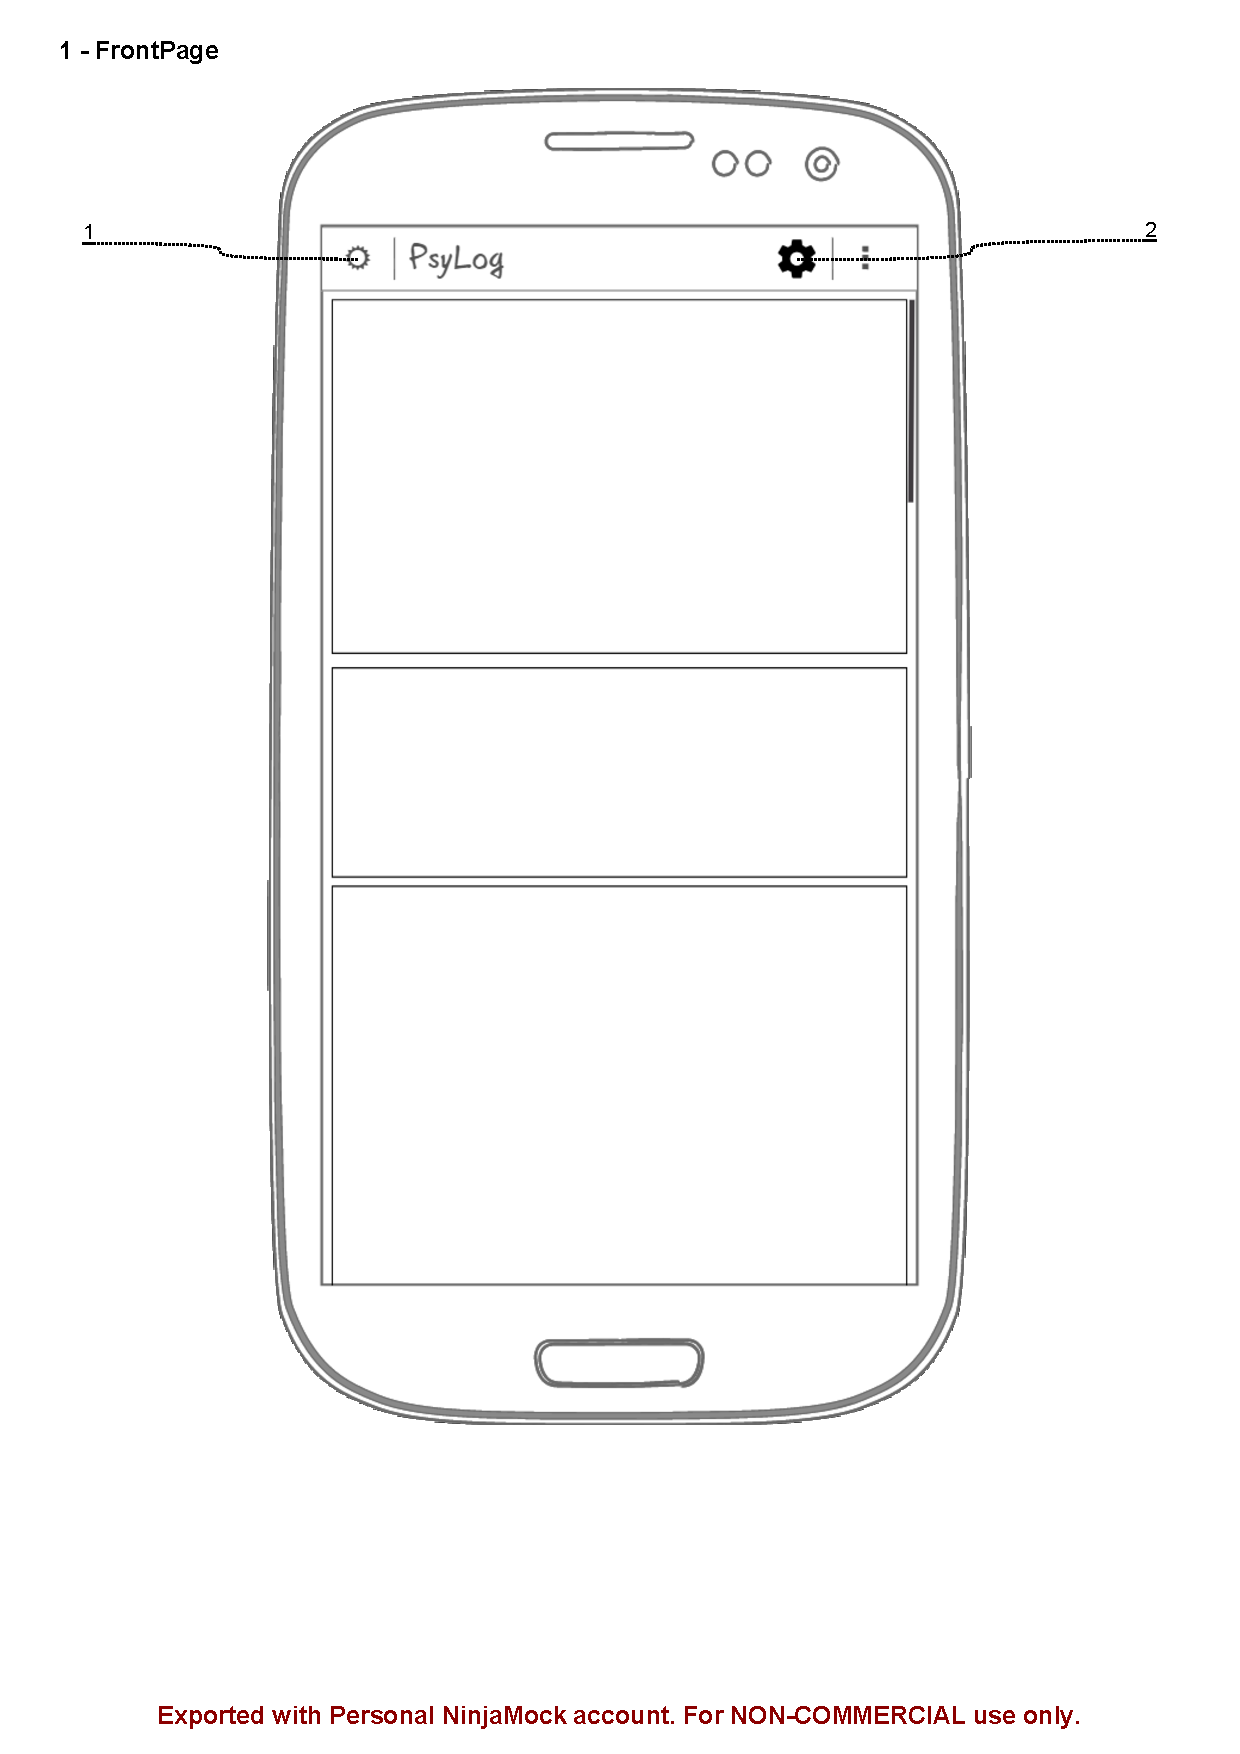
\includegraphics[scale=0.3, page=1, trim = 1cm 5.5cm 1cm 0cm, clip]{prototype.pdf}
			\caption{Forside}
	\end{subfigure}
	\begin{subfigure}[b]{0.45\textwidth}
			\includegraphics[scale=0.3, page=2, trim = 1cm 5.5cm 1cm 0cm, clip]{prototype.pdf}
			\caption{Indstillinger}
	\end{subfigure}
	\caption{Prototype af Manager}
	\label{fig:prototype-manager}
\end{figure}


%Actionbar
Ud fra prototypen kan en actionbar blandt andet ses, tanken er at følge et standard design hvor man har en actionbar i toppen.
Denne muliggør navigation til indstillinger, men også at gå tilbage til hovedmenuen, nuværende er der dog problemer med at den ikke vises under settings\als{Skal have lavet mere arbejde med den}

%Indstillinger, checkbox
Til at angive om et givent modul skal være aktiveret eller ej bruges checkboxes.
Dette skyldes at det er et simpelt ja/nej valg. 
Tanken er så at de moduler man har valgt er dem der kører på telefonen.

%indstillinger, dependencies og events
For at scanne mobilen for de moduler der er installeret bruges JSONParser der tager vare af dette. \als{referer til JSONParser}
Dette giver udslag i en række moduler der har afhængigheder af andre moduler og skal takles.
JSONParseren giver som resultat en liste af moduler. Disse scannes så igennem for at finde deres afhængigheder.
Disse afhængigheder bruges så til at konstruere events (OnChange) til at fortælle de moduler der skal have besked når et givent modul aktiveres/deaktiveres.
Ved at lave en sådan række er der implicit konstrueret en dependency graph.
Og som resultat af dette kan man forestille sig et hierarki hvor et modul på det lavest liggende niveau medfører en kæde af deaktiveringer af moduler der eksplicit og implicit afhænger af dette modul.
\stefan{så vidt jeg ved sker dette ikke længere på samme måde, Winde (eller en der vil sætte sig ind i koden) bør nok revidere dette afsnit}

%indstillinger, onPause start og stop sensorer
Efter afhængighederne er enkodet i programmet mangler der at takle hvordan sensorer skal startes og stoppes fra indstillingsmenuen.
Til at takle dette bruger vi den allerede udviklede ServiceHelper\als{referer til denne}.
Der vælges så at starte og stoppe de fornødne sensorer i onPause, da det typisk er når man forlader en indstillingsmenu at man gerne vil have at indstillingerne træder i kraft, og sikrer også at man ikke skal klikke på ekstra knapper for at indstillingerne træder i kraft.